%%%%%%%%%%%%%%%%%%%%%%%%%%%%%%%%%%%%%%%%%%%%%%%%%%%%%%%%%%%%%%%%%%%%%%%%%%%%%%%
%%
%%          $Id: Rulebook.tex 2014-12-12 balkce $
%%    author(s): RoboCupAtHome Technical Committee(s)
%%  description: introduction to RoboCupAtHome
%%
%%%%%%%%%%%%%%%%%%%%%%%%%%%%%%%%%%%%%%%%%%%%%%%%%%%%%%%%%%%%%%%%%%%%%%%%%%%%%%%
\documentclass[11pt, twoside, openright, a4paper, chapterprefix]{scrbook}
\usepackage[inner=2.5cm, outer=2.5cm, top=4cm, bottom=4cm]{geometry}

%%% PACKAGES %%%%%%%%%%%%%%%%%%%%%%%%%%%%%%%%%%%%%%%%%%%%%%%%%%%%%%%%%%%%%%%%%%
\input{./setup/packages.tex}
\usepackage[titletoc]{appendix}
\usepackage{enumitem}
\usepackage{mathtools}
\usepackage{gensymb}
\setlist{noitemsep}

%%% SubfigureSetup %%%%%%%%%%%%%%%%%%%%%%%%%%%%%%%%%%%%%%%%%%%%%%%%%%%%%%%%%%%%
%\renewcommand{\subfigtopskip}{5pt}        % default is 10pt
%\renewcommand{\subfigbottomskip}{5pt}     % default is 10pt
%\renewcommand{\subfigcapskip}{3pt}        % default is 10pt
%\renewcommand{\subfigcapmargin}{7pt}      % default is 10pt

%%% TweakList-Setup %%%%%%%%%%%%%%%%%%%%%%%%%%%%%%%%%%%%%%%%%%%%%%%%%%%%%%%%%%%
\renewcommand{\itemhook}{%                 % modify itemize-spacing
  \setlength{\topsep}{2pt}%
  \setlength{\partopsep}{1pt}%
  \setlength{\itemsep}{-1pt}%
}
\renewcommand{\enumhook}{%                 % modify enumerate-spacing
  \setlength{\topsep}{2pt}%
  \setlength{\partopsep}{1pt}%
  \setlength{\itemsep}{-1pt}%
}
\renewcommand{\descripthook}{%             % modify description-spacing
  \setlength{\topsep}{2pt}%
  \setlength{\partopsep}{1pt}%
  \setlength{\itemsep}{-1pt}%
}

\setkomafont{title}{\normalfont}
\setkomafont{sectioning}{\normalfont\bfseries}
\addtokomafont{caption}{\small}
\setkomafont{captionlabel}{\small\bfseries}
\setkomafont{descriptionlabel}{\normalfont\bfseries}
\renewcommand*{\chapterformat}{\LARGE{Chapter \thechapter}}

%%% MACROS %%%%%%%%%%%%%%%%%%%%%%%%%%%%%%%%%%%%%%%%%%%%%%%%%%%%%%%%%%%%%%%%%%%%
\input{./setup/active_version.tex}
\graphicspath{{\YEAR/}{./images/}}
\input{./setup/macros.tex}
\input{./setup/abbrevix.tex}



\makeindex                                % generate index
\makeabbex                                % generate abbreviations

%%% DOCUMENTINFO %%%%%%%%%%%%%%%%%%%%%%%%%%%%%%%%%%%%%%%%%%%%%%%%%%%%%%%%%%%%%%
\hypersetup{
  pdftitle     = {RoboCup@Home Rules and Regulations},
  pdfsubject   = {RoboCup@Home Rulebook},
  pdfauthor    = {RoboCup@Home Technical Committee},
  pdfkeywords  = {RoboCup, @Home, Rules, Competition},
  colorlinks   = true,
  anchorcolor  = blue,
  linkcolor    = blue,
  urlcolor     = blue,
}

%%% HEADINGS & PAGE STYLE %%%%%%%%%%%%%%%%%%%%%%%%%%%%%%%%%%%%%%%%%%%%%%%%%%%%%
\newcommand{\footline}{RoboCup@Home Rulebook / \rulebookVersion}
\pagestyle{fancy}
\renewcommand{\chaptermark}[1]{\markboth{\chaptername\ \thechapter. \ #1}{}}
\renewcommand{\sectionmark}[1]{\markright{\thesection \ #1}{}\renewcommand{\currentTest}{#1}}
\fancyhf{}
\fancyhead[LE,RO]{\thepage}
\fancyhead[RE]{\sffamily\rightmark}
\fancyhead[LO]{\sffamily\leftmark}
\fancyfoot[C]{\scriptsize \sffamily \footline{}}
\fancypagestyle{plain}{
        \fancyhf{}
        \fancyhead[LE,RO]{\thepage}
        \fancyhead[RE]{\sffamily\rightmark}
        \fancyhead[LO]{\sffamily\leftmark}
        \fancyfoot[C]{\scriptsize \sffamily \footline{}}
		\renewcommand{\headrulewidth}{0.5 pt}
}
\fancypagestyle{empty}{
        \fancyhf{}
        \fancyhead{}
        \fancyfoot[C]{\scriptsize \sffamily \footline{}}
		\renewcommand{\headrulewidth}{0 pt}
}

\newcommand{\quotes}[1]{``#1''}
\newcommand{\textbi}[1]{\textbf{\textit{#1}}}
%\newcommand{\sectionbreak}{\clearpage}
%\newcommand{\subsectionbreak}{\clearpage}


%%%%%%%%%%%%%%%%%%%\renewcommand{%%%%%%%%%%%%%%%%%%%%%%%%%%%%%%%%%%%%%%%%%%%%%%%%%%%%%%%%%%%%
%%%%%%%%%%%%%%%%%%%%%%%%%%%%%%%%%%%%%%%%%%%%%%%%%%%%%%%%%%%%%%%%%%%%%%%%%%%%%%%
%%%%%%%%%%%%%%%%%%%%%%%%%%%%%%%%%%%%%%%%%%%%%%%%%%%%%%%%%%%%%%%%%%%%%%%%%%%%%%%

\begin{document}

\input{./pages/titlepage}

\pagestyle{empty}
\input{./pages/acknowledgments}
\clearpage

\pagestyle{empty}
\tableofcontents
\clearpage

\pagestyle{plain}

\input{Introduction}

\input{CompetitionConcepts}

\input{GeneralRules}

\input{Setup}

\chapter{Tests in Stage I}
\label{chap:stage_I}

\begin{itshape}
\iterm{Stage~I} comprehends five \textbf{ability tests} and an \textbf{integration test} along with an open demonstration for the audience.
Each ability test is designed to evaluate the average performance of the robot in one particular skill, providing data for benchmarking.
Meanwhile, the integration test has been designed to evaluate how this abilities work together while solving a common task.

The total score for ability and integration tests is the average of the best two performances out of preferably three performances (given the time constraints of a competition).
The point of this is the both elimate good and bad luck for the robots/teams and to get a more objective view of the performance,
  not to give teams time to tweak the robot between test performances.

\iterm{Following and Guiding} (demonstration for the audience) goes out of the arena and into the venue between the audience.

\end{itshape}

\subsection*{Scheduling}
For maximal efficiency, teams will be scheduled interleaved:
  Team A does an attempt while team B sets up their robot. When A is done, it moves out the way for team B, then B attempts while A sets up the robot again etc.

The preparing team should prepare their robot close to the place of the test, but not interfere with the performing robot.
Prepared robots must wait at this preparation location until commanded to start the test.
When commanded to start, the robot must move automatically beyond this point.

Robot should be ready to start the next attempt to the same test as fast as possible:
  when the performing robot is done with a attempt, the next robot must be ready to go with the start of a button or a voice command.

\newpage
\section{Storing Groceries}

The robot must store the groceries on their right place, which is where other objects of the same category are.

\subsection{Goal}
The robot has to correctly identify and manipulate objects at different heights, grouping them by category and likelihood.

\subsection{Focus}
This test focuses on the detection and recognition of objects and their features, as well as object manipulation.

\subsection{Setup}
\begin{enumerate}
\item \textbf{Location:} This test is run in one room of the arena, modified to have a table or trolley (at grasp distance) close to a shelf. The robot will start at a random distance between 1.0m and 1.5m from the bookcase.
\item \textbf{Cupboard:} Any shelf from the arena allocating 10 objects (3 known, 3 alike, 3 unknown, 1 container; see \ref{rule:scenario_objects}) grouped by category and likeliness. 
\item \textbf{Door:} The cupboard has a single door, which is initially closed. At least one object group is accessed through the door.
\item \textbf{Table:} Any table from the arena, having on top 10 shuffled objects (probably stacked, 3 known, 3 alike, 3 unknown, 1 container; see \ref{rule:scenario_objects})
\end{enumerate}

Please note that there may be more than one object in each shelf to fit all objects in, especially after the robot fills the shelves. 

\subsection{Task}
\begin{enumerate}
\item \textbf{Reach the cupboard:} The robot approached to the cupboard (and the table) at grasp distance.
\item \textbf{Inspection:} The robot inspects both, the cupboard and the table.
\item \textbf{Opening door:} The robot opens the cupboard's door and announces which type of objects are stored inside.
\item \textbf{Moving objects:} The robot takes an object from the table and safely places it into the shelf (see Section \refsec{rule:scenario_objects}), close to the other objects in the shelf that belong to the same category. The robot must clearly announce the name and category of the object being moved.
\end{enumerate}

\subsection{Additional rules and remarks}
\begin{enumerate}
  \item \textbf{Startup:} The robot starts with a Start Button (see Section \refsec{rule:start_signal})
  \item \textbf{Collisions:} Slightly touching the the cupboard is tolerated. However, the robot will be stopped immediately if it drives over or smashes the objects/shelf (see section \refsec{rule:safetyfirst}).
  \item \textbf{Cupboard specifications:} The cupboard is any shelf from the arena and has
  \begin{itemize}
    \item[\textbf{DSPL}] At least 3 shelves between 0.90m and 1.50m from the ground.
    \item[\textbf{SSPL}] At least 3 shelves between 0.90m and 1.50m from the ground.
    \item[\textbf{OPL}] At least 5 shelves between 0.30m and 1.80m from the ground.
  \end{itemize}
  \item \textbf{Cupboard's door specifications:} The cupboard has a door that opens outside (i.e., not sliding). The door has a handle or knob is coloured to contrast with the shelve.
  \item \textbf{Recognition report:} Robots must create a report file in PDF format summarizing the the list of recognized objects, and containing the following information:
  \begin{itemize}
    \item A picture of the scene where all recognized objects are labeled and enclosed in a bounding box.
    \item A picture showing each object, it's name/label, and category.
  \end{itemize}

  The report file must be delivered to the TC in a USB-stick after the test. The PDF file name should include the team name and a timestamp.  Objects in the report must be recognizable by a human (TC) so that it can be scored. In case of doubt, no points will be scored.
  \item \textbf{Clear area: } The robot may assume that the direct vicinity of the cupboard and table are clear and that the robot can move slightly backwards for its task. 
\end{enumerate}

\subsection{Data recording}
  Please record the following data (See \refsec{rule:datarecording}):
  \begin{itemize}
   \item Images
   \item Plans
  \end{itemize}

\subsection{OC instructions}

\textbf{2 hours before the test}
\begin{itemize}
    \item Anounce the startup location for robots.
\end{itemize}

\subsection{Referee instructions}
The referee needs to
\begin{itemize}
\item Place the objects in the cupboard and on the table.
\item Shut the cupboard's door.
\end{itemize}

\begin{figure}
  \centering
  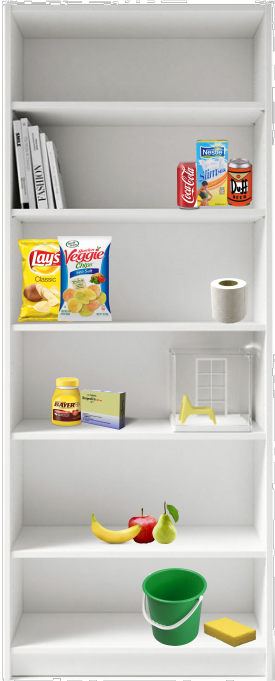
\includegraphics[width=0.25\textwidth]{images/storing_groceries.png}
  \vspace{-10pt}
  \label{fig:storing_groceries}
  \caption{Example shelf where objects will be placed.}
\end{figure}

\subsection{Score sheet}
\section{Storing Groceries}

The robot must store the groceries on their right place, which is where other objects of the same category are.

\subsection{Goal}
The robot has to correctly identify and manipulate objects at different heights, grouping them by category and likelihood.

\subsection{Focus}
This test focuses on the detection and recognition of objects and their features, as well as object manipulation.

\subsection{Setup}
\begin{enumerate}
\item \textbf{Location:} This test is run in one room of the arena, modified to have a table or trolley (at grasp distance) close to a shelf. The robot will start at a random distance between 1.0m and 1.5m from the bookcase.
\item \textbf{Cupboard:} Any shelf from the arena allocating 10 objects (3 known, 3 alike, 3 unknown, 1 container; see \ref{rule:scenario_objects}) grouped by category and likeliness. 
\item \textbf{Door:} The cupboard has a single door, which is initially closed. At least one object group is accessed through the door.
\item \textbf{Table:} Any table from the arena, having on top 10 shuffled objects (probably stacked, 3 known, 3 alike, 3 unknown, 1 container; see \ref{rule:scenario_objects})
\end{enumerate}

Please note that there may be more than one object in each shelf to fit all objects in, especially after the robot fills the shelves. 

\subsection{Task}
\begin{enumerate}
\item \textbf{Reach the cupboard:} The robot approached to the cupboard (and the table) at grasp distance.
\item \textbf{Inspection:} The robot inspects both, the cupboard and the table.
\item \textbf{Opening door:} The robot opens the cupboard's door and announces which type of objects are stored inside.
\item \textbf{Moving objects:} The robot takes an object from the table and safely places it into the shelf (see Section \refsec{rule:scenario_objects}), close to the other objects in the shelf that belong to the same category. The robot must clearly announce the name and category of the object being moved.
\end{enumerate}

\subsection{Additional rules and remarks}
\begin{enumerate}
  \item \textbf{Startup:} The robot starts with a Start Button (see Section \refsec{rule:start_signal})
  \item \textbf{Collisions:} Slightly touching the the cupboard is tolerated. However, the robot will be stopped immediately if it drives over or smashes the objects/shelf (see section \refsec{rule:safetyfirst}).
  \item \textbf{Cupboard specifications:} The cupboard is any shelf from the arena and has
  \begin{itemize}
    \item[\textbf{DSPL}] At least 3 shelves between 0.90m and 1.50m from the ground.
    \item[\textbf{SSPL}] At least 3 shelves between 0.90m and 1.50m from the ground.
    \item[\textbf{OPL}] At least 5 shelves between 0.30m and 1.80m from the ground.
  \end{itemize}
  \item \textbf{Cupboard's door specifications:} The cupboard has a door that opens outside (i.e., not sliding). The door has a handle or knob is coloured to contrast with the shelve.
  \item \textbf{Recognition report:} Robots must create a report file in PDF format summarizing the the list of recognized objects, and containing the following information:
  \begin{itemize}
    \item A picture of the scene where all recognized objects are labeled and enclosed in a bounding box.
    \item A picture showing each object, it's name/label, and category.
  \end{itemize}

  The report file must be delivered to the TC in a USB-stick after the test. The PDF file name should include the team name and a timestamp.  Objects in the report must be recognizable by a human (TC) so that it can be scored. In case of doubt, no points will be scored.
  \item \textbf{Clear area: } The robot may assume that the direct vicinity of the cupboard and table are clear and that the robot can move slightly backwards for its task. 
\end{enumerate}

\subsection{Data recording}
  Please record the following data (See \refsec{rule:datarecording}):
  \begin{itemize}
   \item Images
   \item Plans
  \end{itemize}

\subsection{OC instructions}

\textbf{2 hours before the test}
\begin{itemize}
    \item Anounce the startup location for robots.
\end{itemize}

\subsection{Referee instructions}
The referee needs to
\begin{itemize}
\item Place the objects in the cupboard and on the table.
\item Shut the cupboard's door.
\end{itemize}

\begin{figure}
  \centering
  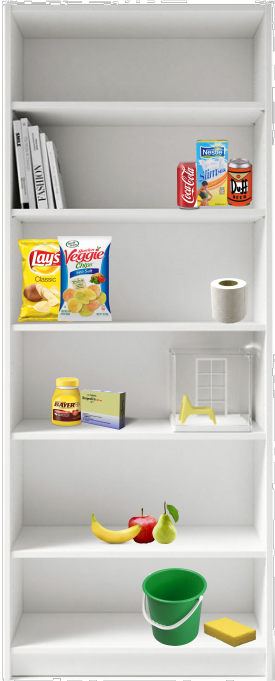
\includegraphics[width=0.25\textwidth]{images/storing_groceries.png}
  \vspace{-10pt}
  \label{fig:storing_groceries}
  \caption{Example shelf where objects will be placed.}
\end{figure}

\subsection{Score sheet}
\section{Storing Groceries}

The robot must store the groceries on their right place, which is where other objects of the same category are.

\subsection{Goal}
The robot has to correctly identify and manipulate objects at different heights, grouping them by category and likelihood.

\subsection{Focus}
This test focuses on the detection and recognition of objects and their features, as well as object manipulation.

\subsection{Setup}
\begin{enumerate}
\item \textbf{Location:} This test is run in one room of the arena, modified to have a table or trolley (at grasp distance) close to a shelf. The robot will start at a random distance between 1.0m and 1.5m from the bookcase.
\item \textbf{Cupboard:} Any shelf from the arena allocating 10 objects (3 known, 3 alike, 3 unknown, 1 container; see \ref{rule:scenario_objects}) grouped by category and likeliness. 
\item \textbf{Door:} The cupboard has a single door, which is initially closed. At least one object group is accessed through the door.
\item \textbf{Table:} Any table from the arena, having on top 10 shuffled objects (probably stacked, 3 known, 3 alike, 3 unknown, 1 container; see \ref{rule:scenario_objects})
\end{enumerate}

Please note that there may be more than one object in each shelf to fit all objects in, especially after the robot fills the shelves. 

\subsection{Task}
\begin{enumerate}
\item \textbf{Reach the cupboard:} The robot approached to the cupboard (and the table) at grasp distance.
\item \textbf{Inspection:} The robot inspects both, the cupboard and the table.
\item \textbf{Opening door:} The robot opens the cupboard's door and announces which type of objects are stored inside.
\item \textbf{Moving objects:} The robot takes an object from the table and safely places it into the shelf (see Section \refsec{rule:scenario_objects}), close to the other objects in the shelf that belong to the same category. The robot must clearly announce the name and category of the object being moved.
\end{enumerate}

\subsection{Additional rules and remarks}
\begin{enumerate}
  \item \textbf{Startup:} The robot starts with a Start Button (see Section \refsec{rule:start_signal})
  \item \textbf{Collisions:} Slightly touching the the cupboard is tolerated. However, the robot will be stopped immediately if it drives over or smashes the objects/shelf (see section \refsec{rule:safetyfirst}).
  \item \textbf{Cupboard specifications:} The cupboard is any shelf from the arena and has
  \begin{itemize}
    \item[\textbf{DSPL}] At least 3 shelves between 0.90m and 1.50m from the ground.
    \item[\textbf{SSPL}] At least 3 shelves between 0.90m and 1.50m from the ground.
    \item[\textbf{OPL}] At least 5 shelves between 0.30m and 1.80m from the ground.
  \end{itemize}
  \item \textbf{Cupboard's door specifications:} The cupboard has a door that opens outside (i.e., not sliding). The door has a handle or knob is coloured to contrast with the shelve.
  \item \textbf{Recognition report:} Robots must create a report file in PDF format summarizing the the list of recognized objects, and containing the following information:
  \begin{itemize}
    \item A picture of the scene where all recognized objects are labeled and enclosed in a bounding box.
    \item A picture showing each object, it's name/label, and category.
  \end{itemize}

  The report file must be delivered to the TC in a USB-stick after the test. The PDF file name should include the team name and a timestamp.  Objects in the report must be recognizable by a human (TC) so that it can be scored. In case of doubt, no points will be scored.
  \item \textbf{Clear area: } The robot may assume that the direct vicinity of the cupboard and table are clear and that the robot can move slightly backwards for its task. 
\end{enumerate}

\subsection{Data recording}
  Please record the following data (See \refsec{rule:datarecording}):
  \begin{itemize}
   \item Images
   \item Plans
  \end{itemize}

\subsection{OC instructions}

\textbf{2 hours before the test}
\begin{itemize}
    \item Anounce the startup location for robots.
\end{itemize}

\subsection{Referee instructions}
The referee needs to
\begin{itemize}
\item Place the objects in the cupboard and on the table.
\item Shut the cupboard's door.
\end{itemize}

\begin{figure}
  \centering
  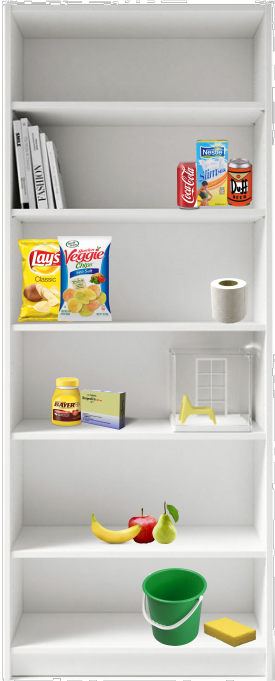
\includegraphics[width=0.25\textwidth]{images/storing_groceries.png}
  \vspace{-10pt}
  \label{fig:storing_groceries}
  \caption{Example shelf where objects will be placed.}
\end{figure}

\subsection{Score sheet}
\input{scoresheets/StoringGroceries.tex}

% Local Variables:
% TeX-master: "Rulebook"
% End:


% Local Variables:
% TeX-master: "Rulebook"
% End:


% Local Variables:
% TeX-master: "Rulebook"
% End:


\newpage
\input{tests/Navigation}

\newpage
\input{tests/PersonRecognition}

\newpage
\input{tests/SpeechRecognition}

\newpage
\section{Help-me-carry}
The robot's owner went shopping for groceries and needs help carrying the groceries from the car into the home.
The whole family helps, as well as the robot. 

\subsection{Goal}
The robot must bring some items from outside the arena inside the arena.

\subsection{Focus}
This test focuses on following and navigation in an unknown environment. 

\subsection{Setup}
The robot starts waiting inside the arena. 
The operator (the robot's owner) has a set of bags and boxes that need to be carried from a place outside the arena back inside. 

\begin{enumerate}
  \item \textbf{Location:} One of the arenas (apartment) and its surroundings. The apartment is in its normal state. Part of the test is performed outside the arena in a public space.
  \item \textbf{Start:} Starting location of the robot. %%Close *to* the front door of the appartment?
  \item \textbf{Car:} The robots operator has put the groceries in the trunk of the car after shopping. The car is parked outside the home.
  \item \textbf{Destinations:} The items must be transported to places where they can be stored. The destinations are various rooms of the arena. 
  \item \textbf{Doors:} All doors in the apartment are open.
  \item \textbf{Operator:} A \quotes{professional} operator is selected by the TC to act as the operator of the robot. 
  \item \textbf{Other people:} There are no restrictions on other people walking by or standing around throughout the complete task. 
\end{enumerate}

\subsection{Task (OPL \& DSPL)}
\begin{enumerate}
\item \textbf{Start:} The robot is waiting somewhere in the apartment. The operator approaches the robot and tells it to follow. E.g. ``Robot, follow me''
\item \textbf{Following:} The robot starts following the operator, who guides the robot to the car containing the groceries. 
\item \textbf{Arrive at car:} When at the car, the operator tells the robot they have reached the car and to remember this location. E.g. ``Remember: this location is the car''. 
\item \textbf{Handover groceries:} The operator gives the robot a command to carry something, e.g. a box or a bag.  E.g. ``Carry this box''
  The robot puts up its arms and the operator gives the item to the robot.
\item \textbf{Command destination:} The operator tells where the given item should go, one of the rooms in the arena. E.g. ``Bring this to the kitchen''
\item \textbf{Delivery:} The robot then goes inside the house to deliver the item to the destination. 
\item \textbf{Guiding:} Close to the destination, a human will be waiting. The robot must ask the human for help in carrying stuff and the robot must guide that helping human to the car.
\end{enumerate}

\subsection{Task (SSPL)}
\begin{enumerate}
	\item \textbf{Start:} The robot is waiting somewhere in the apartment. The operator approaches the robot and tells it to follow. E.g. ``Robot, follow me''
	\item \textbf{Following:} The robot starts following the operator, who guides the robot to the car containing the groceries. 
	\item \textbf{Arrive at car:} When at the car, the operator tells the robot they have reached the car and to remember this location. E.g. ``Remember: this location is the car''. 
	\item \textbf{Asked for help:} The operator gives the robot a command to find help for unloading the car.  E.g. ``Ask Gary in the kitchen to help me''.
	The robot must go find a person in the commanded room. 
	\item \textbf{Asking for help:} The robot asks the person for help with carrying stuff.
	\item \textbf{Guiding:} The robot then guides the helper to the car.
\end{enumerate}

The robot may encounter some obstacles while navigating and the robot must deal and avoid or otherwise deal with the obstacle. 
The possible obstacles are:
\begin{itemize}
	\item \textbf{Small object:} Small object. For example, someone has dropped a piece of fruit (like an apple or mandarin) while carrying the groceries inside.
	\item \textbf{3D Object:} A bar table, normal table, rolling chair: some object that is wider at its top than on its bottom, 
	  thus requiring more than just a laser scanner mounted near the ground to avoid obstacles. 
	\item \textbf{Smart obstacle:} A person to whom the robot may speak to and kindly ask to move away. 
	  When interacting with people, the robot must look at the person and make clear is speaking with him/her.
	\item \textbf{Moving people:} As the whole family living in the house is helping getting the groceries from the car, 
	  additional to the robot there will be some people also going back and forth between the car and various rooms. 
	  The robot will encounter these and deal with them. These people are friendly to the robot and will not actively block it but the robot must also not block them. 
\end{itemize}
%% Possible extensions: 
%% - DONE: allow the operator to tell for each item where it should go
%% - At the destination room, there is a person waving, waiting for the robot to bring the items so (s)he can take them
%% - Points for a natural handover. E.g. the human is holding a box and the robot moves in to take it over instead of the humans placing it in the robots arms. Same for the bag
%% - Close the appartment door when the robot is inside?

\subsection{Additional rules and remarks}
\begin{enumerate}
  \item \textbf{Delivering items:} At the destination, the robot may place the bag or box at a convenient location: the floor or a table
  \item \textbf{Obstacle avoidance:} The robot will encounter some human(s) on the way between the two locations.  
\end{enumerate}

\subsection{Data recording}
  Please record the following data (See \refsec{rule:datarecording}):
  \begin{itemize}
   \item Maps
   \item Plans
  \end{itemize}

\subsection{Referee instructions}

The referee needs to
\begin{itemize}
\item Distribute some objects over some boxes and shopping bags.
\item Destignate a few ``car parking locations'' from which the objects must be carried.
\end{itemize}

\subsection{Score sheet}

The maximum time for this test is 6 minutes.

\begin{scorelist}
	\scoreheading{Single iteration}
	\scoreitem{10}{Reach the car}
	\scoreitem{20}{Natural handover to accept the item from the owner}
	\scoreitem{5}{Understand the commanded destination}
	\scoreitem{10}{Reach inside the arena again}
	\scoreitem{10}{Reach the destination}
	\scoreitem{5}{Put the item at the floor or a nearby table}
	% 3x 60 points = 180 only
	
	% Up to 60 points
	\scoreheading{Dealing with obstacles}
	\scoreitem{5}{Avoiding small object}
	\scoreitem{10}{Avoiding 3D object (Difficult-to-see object)}
	\scoreitem{5}{Asking a person to step aside}
	\scoreitem{30}{Moving away movable object}
	\scoreitem{10}{Move aside for person}
	\scoreitem{50}{Open closed door}
	
	\setTotalScore{290}
\end{scorelist}


% Local Variables:
% TeX-master: "Rulebook"
% End:


\chapter{Tests in Stage II}
\label{chap:stage_II}

\begin{itshape}
All ability and integration tests in \iterm{Stage~II} grants 250 points (but the \iterm{Open Challenge} which grants 250) and are performed only once. Some tests have optional tasks that grant additional points when performed correctly, clean and fast. The \iaterm{Technical Committee}{TC} must be informed if a team is planning to perform any of the optional tasks. Unless explicitly stated otherwise, no additional time is given while performing optional tasks.

In the \iterm{Open Challenge} the robot must be able to show to the \iaterm{Technical Committee}{TC} the achievements on the main research line of its own team. This test grants up to 200 points.

\section{Robot \& team cooperation}
We encourage robots and teams to work together when performing challenges.
For scoring, points are awarded per subtask. The robot (and thus team) performing the subtask gets the points.
For example, in the Restaurant-challenge, if one robot of team A can take the order and another robot of team B delivers the order, then the points for taking the order go to team A, while the points for delivering go to team B.
Of course, team A \& B can both perform the challenge in their own turn.

\end{itshape}

\newpage
\input{tests/TidyUp}

\newpage
\input{tests/OpenChallenge}

\newpage
\input{tests/Restaurant}

\newpage
\input{tests/EEGPSR}

\newpage
\input{tests/Finals}

\input{Appendices}

\printabx
\printidx

\end{document}
